Cuando se coloca una carga \(q\) en un campo eléctrico \(\vec{E}\), la carga experimenta una fuerza \(\vec{F}=q\vec{E}\). Esta fuerza es conservativa, lo que significa que el trabajo realizado por la fuerza al mover la carga entre dos puntos \(A\) y \(B\) no depende de la trayectoria seguida, sino solo de los puntos inicial y final.

El trabajo realizado por la fuerza al mover la carga \(q\) desde el punto \(A\) hasta el punto \(B\) se define como:
\begin{equation*}
    W_{AB} = \int_A^B \vec{F} \cdot d\vec{s} = \int_A^B q\vec{E} \cdot d\vec{s}
\end{equation*}

donde \(d\vec{s}\) es un elemento diferencial de desplazamiento a lo largo de la trayectoria. Y como la fuerza eléctrica es conservativa, podemos expresarla en términos de la energía potencial eléctrica \(U\):

\begin{equation*}
    W_{AB} = U_A - U_B = -\Delta U
\end{equation*}

\subsubsection{Definición de potencial eléctrico}

Para una posición conocida de la carga de prueba en el campo, el sistema carga-campo tiene una energía potencial \(U\) relativa a la configuración del sistema definida como \(U=0\). Al dividir la energía potencial entre la carga de prueba \(q\), obtenemos el \textbf{potencial eléctrico} \(V\) en un punto \(P\) del campo eléctrico:

\begin{equation}
    V = \frac{U}{q}
    \label{eq:potential}
\end{equation}

El potencial eléctrico es una magnitud escalar que se mide en \(\text{V}\) (voltios) y se define como la energía potencial por unidad de carga.

Teniendo en cuenta la definición de potencial (ecuación \eqref{eq:potential}) la \textbf{diferencia de potencial} \(\Delta V = V_B - V_A\) entre dos puntos \(A\) y \(B\) en un campo eléctrico se define como el cambio en energía potencial por unidad de carga al mover una carga de prueba \(q\) entre esos dos puntos:

\begin{equation}
    \Delta V = \frac{\Delta U}{q} = -\int_A^B \vec{E} \cdot d\vec{s}
    \label{eq:potential_difference}
\end{equation}

Por la ecuación \eqref{eq:potential_difference}, el trabajo realizado por un agente externo al desplazar una carga \(q\) a través de un campo eléctrico con una velocidad constante es:

\[
W=q\Delta V
\]

Es muy importante que el desplazamiento de la carga \(q\) sea a velocidad constante, ya que si no lo es, el trabajo realizado por el agente externo no será igual al trabajo realizado por la fuerza eléctrica. 

Nótese que el concepto de potencial eléctrico se concive de forma similar al de campo eléctrico. Se usa una carga de prueba positiva \(q\) haciendo que sólo dependa de la carga fuente \(Q\) que genera el campo eléctrico. 

\subsubsection{Diferencia de potencial en un campo eléctrico uniforme}

La ecuación \eqref{eq:potential_difference} es válida en todos los campos eléctricos, sean uniformes o no. En un campo eléctrico uniforme, la magnitud del campo \(\vec{E}\) es constante y la dirección de \(\vec{E}\) es la misma en todos los puntos del campo. En este caso, la diferencia de potencial entre dos puntos \(A\) y \(B\) separados por una distancia \(d\) en la dirección del campo eléctrico se puede expresar como:
\begin{equation}
    \Delta V = -\int_A^B \vec{E} \cdot d\vec{s} = -E \, \int_A^B ds = \boxed{-Ed}
    \label{eq:potential_uniform}
\end{equation}
donde \(E\) es la magnitud del campo eléctrico y \(d\) es la distancia entre los puntos \(A\) y \(B\) en la dirección del campo.

El signo negativo indica que el potencial en el punto \(B\) es menor que el potencial en el punto \(A\) si la carga de prueba se mueve en la dirección del campo eléctrico. Esto significa que el trabajo realizado por la fuerza eléctrica es negativo, lo que implica que la energía potencial disminuye al mover la carga en la dirección del campo eléctrico.

\begin{figure}[ht]
    \centering
    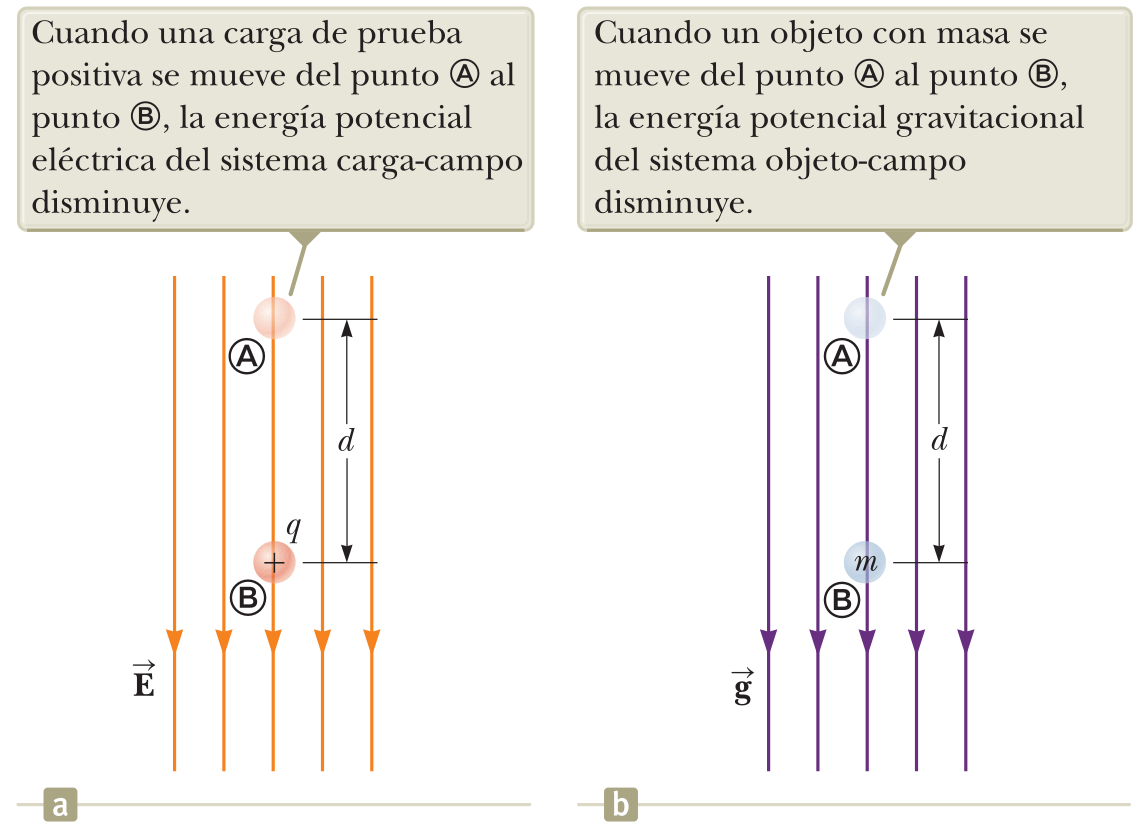
\includegraphics[width=0.8\textwidth]{potential_const_field.png}
    \caption{Comparación de la energía potencial eléctrica y gravitatoria.}
    \label{fig:potential_uniform}
\end{figure}

\begin{tcolorbox}[mydanger]
    CUIDADO: si la carga \(q\) es negativa, la situación se invierte. El sistema gana energía potencial al mover la carga \(q\) en la dirección del campo eléctrico, y disminuye al moverla en la dirección opuesta.    
\end{tcolorbox}

\subsubsection{Potencial eléctrico debido a una carga puntual}

\begin{wrapfigure}{l}{0.32\textwidth}
    \centering
    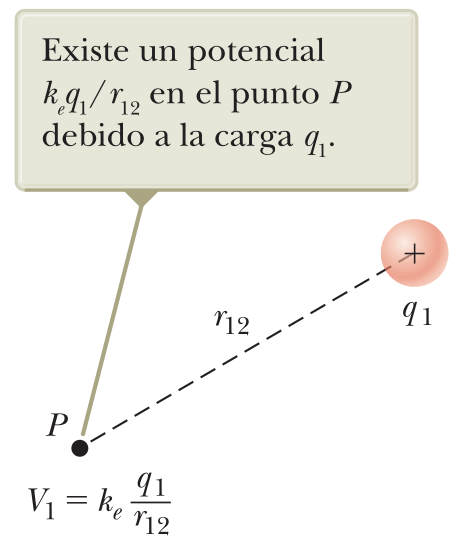
\includegraphics[width=0.33\textwidth]{puntual_potential_1.png}
    \caption{Potencial en el punto \(P\) debido a \(q_1\).}
    \label{fig:potential_point_charge}
\end{wrapfigure}

Como se mensiona en la definición, la energía potencial es relativa al punto que se ha definido como ``0''. Con  el potencial eléctrico pasa lo mismo, entonces si queremos saber el potencial en un punto \(P\) del campo eléctrico, sabemos que es igual al trabajo realizado por la fuerza eléctrica al mover una carga de prueba \(q\), pero ¿Desde donde hasta donde? Bueno, podemos definir que nuestro potencial sea cero cuando la carga \(q\) esté infinitamente alejada de la fuente. Entonces el potencial en el punto \(P\) es trabajo para mover la carga de prueba desde el infinito hasta el punto \(P\):

\begin{align*}
    V_P &= - \lim_{a \to \infty}\int_{a}^P \vec{E} \cdot d\vec{r}\\
        &= - \lim_{a \to \infty}\int_{a}^P \frac{kq_1}{r^2} \cdot dr\\
        &= -kq_1 \, \lim_{a \to \infty} \int_{a}^P \frac{1}{r^2} \cdot dr\\
        &= -kq_1 \, \lim_{a \to \infty} \left[ -\frac{1}{r} \right]_{a}^P\\
        &= -kq_1 \, \lim_{a \to \infty} \left[ -\frac{1}{P} + \frac{1}{a} \right]\\
        &= -kq_1 \, \left[ -\frac{1}{P} + 0 \right] \\
    V_P &= k\frac{q_1}{r_{12}} = \lVert\vec{E}\rVert \, \lVert\vec{r}_{12}\rVert \cos(0)
\end{align*}
por ser \(\vec{E}\) y \(\vec{r}_{12}\) paralelos. Entonces el potencial eléctrico en un punto \(P\) debido a una carga puntual \(q_1\) es:
\begin{equation}
    \boxed{V_P = k\frac{q_1}{r_{12}} = E \, r_{12}}
    \label{eq:potential_point_charge}
\end{equation}

donde \(q_1\) es la carga fuente, \(E\) el campo generado por \(q_1\) y \(r_{12}\) la distancia a un punto en el campo eléctrico.

El potencial eléctrico debido a múltiples cargas puntuales se basa en el principio de superposición, que establece que el potencial eléctrico total en un punto es igual a la suma algebraica de los potenciales individuales producidos por cada carga.

\begin{equation}
    V_{total} = \sum_{i=1}^{n} V_i = k \sum_{i=1}^{n} \frac{q_i}{r_i}
\end{equation}

\subsubsection{Obtención de \(\vec{E}\) a partir de \(V\)}

El campo eléctrico \(\vec{E}\) y el potencial eléctrico \(V\) están relacionados, como se muestra en la ecuación \eqref{eq:potential_point_charge}, que se usa para encontrar \(V\) en un punto cuando se conoce \(\vec{E}\). Sin embargo, también podemos encontrar \(\vec{E}\) a partir de \(V\) usando la relación:

\begin{equation}
    dV = -\vec{E} \cdot d\vec{s}
    \label{eq:field_from_potential_differential}
\end{equation}

y si estamos trabajando con una única coordenada podemos escribir la ecuación \eqref{eq:field_from_potential_differential} como:

\[
    dV = -E \, ds \quad \Rightarrow \quad E = -\frac{dV}{ds}
\]

Sin embargo, en general, el potencial eléctrico es una función de las tres coordenadas espaciales. Si \(V(r)\) se da en coordenadas cartesianas, las componentes \((E_x, E_y, Ez)\) del campo eléctrico pueden ser determinadas fácilmente a partir de \(V(x, y, z)\) como derivadas parciales

\begin{equation}
    \vec{E} = -\nabla V
    \label{eq:field_from_potential}
\end{equation}
donde \(\nabla\) es el operador nabla, que representa el \hl{gradiente del potencial eléctrico}. Esta relación indica que el campo eléctrico es igual al negativo del gradiente del potencial eléctrico. En otras palabras, el campo eléctrico apunta en la dirección de mayor disminución del potencial eléctrico.

\paragraph{Recordatorio: operador nabla}

El operador \textbf{nabla} (\(\nabla\)), también conocido como \textbf{operador del gradiente}, es una herramienta matemática usada en cálculo vectorial y análisis multivariable. Se utiliza para representar derivadas en múltiples dimensiones.

Formalmente, el operador nabla se define como:

\[
\nabla = \left( \frac{\partial}{\partial x}, \frac{\partial}{\partial y}, \frac{\partial}{\partial z} \right)
\]

Es un operador vectorial que, aplicado a diferentes tipos de funciones, da lugar a distintos conceptos:

\subparagraph{Gradiente}

Cuando se aplica a una función escalar \( f(x, y, z) \), produce un \textbf{campo vectorial} que apunta en la dirección de mayor incremento de la función. Se expresa como:

\[
\nabla f = \left( \frac{\partial f}{\partial x}, \frac{\partial f}{\partial y}, \frac{\partial f}{\partial z} \right)
\]

Este vector resultante indica la dirección en la que la función crece más rápidamente y su magnitud corresponde a la tasa de cambio máxima. En el caso de \(\vec{E}\) y \(V\), \(\vec{E}\) es el gradiente de \(V\) representa una función vectorial que apunta en la dirección de mayor aumento del potencial eléctrico.

\subparagraph{Divergencia}

Cuando se aplica a un campo vectorial \( \vec{F} = (F_x, F_y, F_z) \), el operador nabla actúa como un producto escalar:

\[
\nabla \cdot \vec{F} = \frac{\partial F_x}{\partial x} + \frac{\partial F_y}{\partial y} + \frac{\partial F_z}{\partial z}
\]

\subparagraph{Rotacional}

Cuando se aplica a un campo vectorial, el operador nabla actúa como un producto cruz:

\[
\nabla \times \vec{F}
\]

